\chapter{Contributions to Spot}

This chapter present the different things I have done on Spot during the internship. Might it be
some algorithms implemented, scripts, display arrangements, benchmarks, results analyzes, etc.

\noindent All the achieved work is presented in a chronological way, to bring out the difficulties
encountered, the unexpected results that had influence on the advancement of the work.

\section{fastSAT}
As a quick reminder, here are the required characteristics for the SAT solver:
\begin{itemize}
 \item licence compatibility with Spot's one (GNU GPL v3),
 \item simplicity of integration for future updates,
 \item effectiveness.
\end{itemize}

\noindent The project \textbf{fastSAT}\cite{5} was born to help choose the SAT solver to distribute with
Spot. Until now, SAT-based minimization was performed through an external SAT solver. The default one
was Glucose \cite{12} (3.0 version). Therefore, it seems logical to consider Glucose as a possible
candidate. \textbf{fastSAT}\cite{5} compared Glucose 4.0 \cite{12} to CryptoMiniSat 5.0.1\cite{20} and
PicoSAT 965 \cite{21}. Note that some SAT solvers provide two versions, one parallal and one simple
essentially because of the SAT competitions. In short, were compared:
\begin{itemize}
 \item Glucose syrup (parallal) 4.0
 \item Glucose simple 4.0
 \item CryptoMiniSat parallal 5.0.1
 \item CryptoMiniSat simple 5.0.1
 \item PicoSAT 965
\end{itemize}

The next three figures (\ref{fig:satchoose_1}, \ref{fig:satchoose_2} and \ref{fig:satchoose_3}) show some
comparaisons for three formulas. About twenty formulas have been tested in two modes: by forcing the number
of state and by doing the complete cycles of minimization. It has been executed on a computer with an
\textbf{Intel(R) Core(TM) i7-4710HQ CPU @ 2.50GHz} processor and  a \textbf{8 GiB} system memory.
The measuring tool used is the open Google Benchmark tool \cite{22}.

\begin{figure}[H]
 \centering
 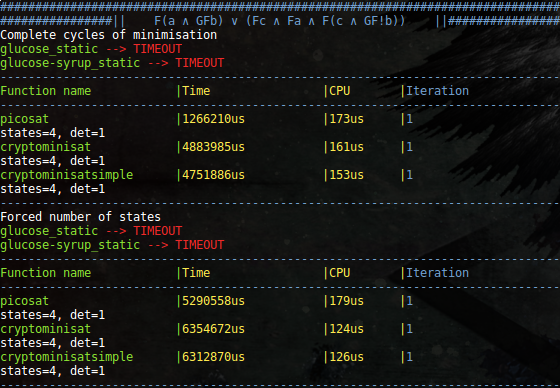
\includegraphics[scale=0.7]{img/satchoose_1.png}
 \caption{Benchmark for formula $F(a \land GFb) \lor (Fc \land Fa \land F(c \land GF(!b)))$}
 \label{fig:satchoose_1}
\end{figure}

\begin{figure}[H]
 \centering
 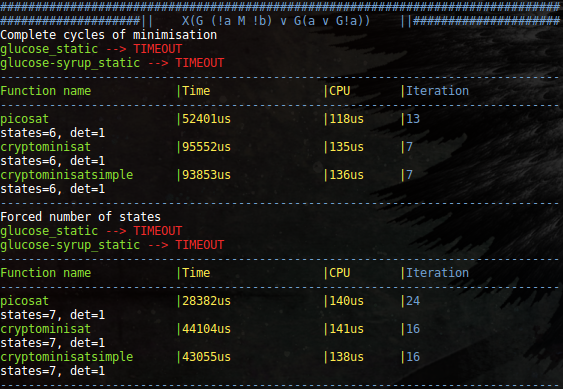
\includegraphics[scale=0.7]{img/satchoose_2.png}
 \caption{Benchmark for formula $X(G (!a M !b) \lor G(a \lor G(!a)))$}
 \label{fig:satchoose_2}
\end{figure}

\begin{figure}[H]
 \centering
 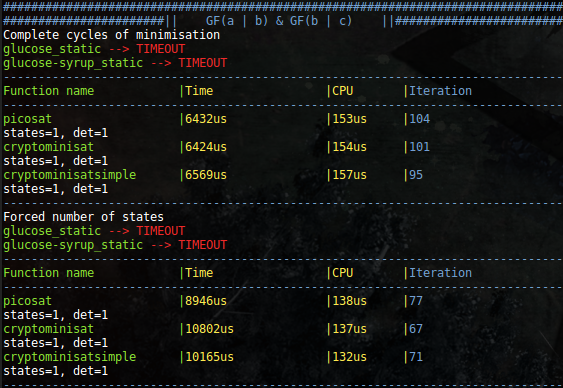
\includegraphics[scale=0.7]{img/satchoose_3.png}
 \caption{Benchmark for formula $GF(a \lor b) \land GF(b \lor c)$}
 \label{fig:satchoose_3}
\end{figure}

\noindent In conclusion, among the different SAT solvers, \textbf{PicoSAT} was choosen for its strong
performances. It consists of two source code files: \textbf{picosat.h} and \textbf{picosat.c} and was
easily integrated and harmonised with Spot.

\textbf{fastSAT}\cite{5} project is fully availlable and anyone can reproduce the benchmarks. Feel free to
have a look.

\section{New Satsolver class}
There was already a satsolver class that is instantiated at the beginning of the SAT-based minimization
procedures, formerly used to initialize a temporary \textbf{cnf file} (DIMACS \cite{18}), return
it and call the external SAT solver. The file writing was directly made by those procedures.

\noindent The objective is to completely abstract the file writing. SAT-based minimization procedures will
just have to instantiate a satsolver object at the beginning and make calls to its functions. Thoses
functions will call the SAT solving library functions. But this class must continue to support any external
SAT solver by handling temporary \textbf{cnf files}.\\

\begin{figure}[h]
  \centering
  \begin{tikzpicture}
    \begin{umlpackage}{Pseudo UML}
     \umlclass[name=satsolver, template=T]{spot::satsolver}
     {
       psat\_ : PicoSAT*\\
       cnf\_stream\_ : std::ostream*\\
       nb\_clauses\_ : int\\
       nb\_vars\_ : int\\
       ...
       }{
       add(std::initializer\_list\textless int\textgreater values : void\\
       add(int v) : void\\
       comment(T first, Args... args)\\
       get\_nb\_clauses() : int\\
       get\_nb\_vars() : int\\
       get\_solution() : std::pair\textless int, std::vector\textless bool\textgreater\textgreater\\
       ...
     }
    \end{umlpackage}
  \end{tikzpicture}
  \caption{Satsolver class UML representation}
  \label{fig:sat_uml}
\end{figure}

\noindent The figure \ref{fig:sat_uml} shows an approximate UML representation of the new satsolver class.
It can either initialize PicoSAT or a cnf\_stream\_. The idea is to let its functions (add, comment, etc.)
to decide if they call PicoSAT functions or write in the cnf\_stream\_. That way, SAT-based minimization
procedures are not aware of what's going on behind and can repeat over and over again the same algorithms.\\

\noindent Of course the clause counting mechanism is provided by the new satsolver class. At the end,
SAT-based procedures will just have to call the \textit{get\_solution()} method.\\

Once this was done, SAT-based procedures had already gained some speed which is entirely understandable as
disk operations are slow. For instance, with this command
line:
\begin{lstlisting}[language=bash,caption={bash command-line to test a formula minimization using ltl2tgba}]
  time ltl2tgba -D -x sat-minimize 'G(a -> Fb) & G(c -> Fd)'
                        --stats='states=%s, det=%d’
\end{lstlisting}
This result is obtained on a Macbook pro with \textbf{2,9GHz intel core i5} and
\textbf{8 Go 1867 Mhz DDR3}:\\\\
\begin{tabular}{|c|c|}
 \hline
 &\\
 PicoSAT as & Time result\\
 &\\
 \hline
 &\\
 linked SAT solving library&0.29s user 0.08s system 98\% cpu 0.371 total\\
 external SAT solver (with disk operations)&0.82s user 0.09s system 98\% cpu 0.925 total\\
 &\\
 \hline
\end{tabular}

\section{First incremental approach}
Just as a reminder, until now, SAT-based minimization procedures whether it is with binary search
(algorithm \ref{dicho}) or the naive way (algorithm \ref{naive}), starts the SAT encoding from scratch
at each step of the cycle of minimization; that is unfortunate. This is why an incremental approach
has been considered.\\

\noindent  The algorithm \ref{incr1} has been implemented. Starting with an $\omega$-automaton of size
$n$, if the first iteration (which encodes the research of an $\omega$-automaton of size $n-1$) constructs
an automaton of $k$ ($k \leq n-1$) states \textit{accessible}, then some clauses are added to forbid all the
entrant transitions of the $n-k-1$ last state. If such automaton is found, the entrant transitions of the
$n-k-2$ last state are also forbidden, etc. The last SAT problem solved correspond to the minimal
automaton.\\

\noindent An interesting thing, as a sideline, is that at the beginning, instead of forbidding the entrant
transitions of a state, the outgoing transitions were forbidden. This did not work, because those
clauses were in contradiction with the first rule of the encoding (which stated that the automaton must be
\textit{complete}), causing an absurdity. All the rules of the encoding are described in the papers
\cite{14} and \cite{15}.\\

\noindent After this method has been implemented (algorithm \ref{incr1}), a benchmark has been realized to
compare it to the old default method (algorithm \ref{naive}). For dispay reasons, only a few interesting
lines of the results are displayed in the figure \ref{fig:glu_vs_incr1_short}. Feel free to have a look
in the \ref{glu_vs_incr1_complete} section of the appendix to see all the results. For each version and
each formula, two minimizations are attempted, büchi \textit{acceptance set} and
\textit{generalized büchi acceptance set}. The best performances for each formula are colorized
respectively in green and yellow.

\begin{figure}[H]
 \centering
 \fontsize{9}{11}\selectfont{
 \setlength\LTleft{0pt}% default: \parindent
 \setlength\LTright{0pt}% default: \fill
 \begin{longtable}{@{\extracolsep{\fill}}|*{5}{c|}}
  \hline
  \multirow{3}{*}{Formulas}&\multicolumn{4}{c|}{Time (seconds)}\\
  &\multicolumn{2}{c|}{Glucose (As before)}&\multicolumn{2}{c|}{Incr Naive}\\
  &minDBA&minDTGBA&minDBA&minDTGBA\\
  \hline
  $F(a \land  GFb) \lor  (Fc \land  Fa \land  F(c \land  GF\bar b))$&0.02&\cellcolor{Yelw} 57.65&\cellcolor{Green} 0.01&236.36\\
  $XXG(Fa U Xb)$&25.15&\cellcolor{Yelw} 762.74&\cellcolor{Green} 20.21&(killed)\\
  $(a R (b R Fc)) W XGb$&(killed)&\cellcolor{Yelw} 254.19&(killed)&672.80\\
  $X(\bar a \land  Fa) R (a M Fb)$&2.19&\cellcolor{Yelw} 46.12&\cellcolor{Green} 1.7&132.02\\
  $(a R Fb) U X\bar c$&(killed , $\le$ 11)&\cellcolor{Yelw} 389.87&(killed , $\le$ 11)&616.70\\
  \hline
 \end{longtable}}
 \caption{Parts of \ref{glu_vs_incr1_complete} benchmark results showing some cases where the Old SAT-based
          minimization is still better}
 \label{fig:glu_vs_incr1_short}
\end{figure}

In all the lines of the figure \ref{fig:glu_vs_incr1_short}, \textbf{glucose} is still better than our first
incremental approach. There is even a case where \textbf{naive incr} never ends the minimization and
is killed.

In order to better compare both version, this generated figure counts the number of times a version is better
than the other with a tolerance of more or less five percents (5\%). That means roughly equal times are skipped.
\begin{figure}[H]
 \centering
 \begin{tabular}{|c|c|c|c|}
\hline
\multicolumn{4}{|c|}{DBA}\\
\hline
&glu&incr1&total\\
\hline
glu&{-}&9&9\\
\hline
incr1&102&{-}&102\\
\hline
\multicolumn{4}{c}{}\\
\hline
\multicolumn{4}{|c|}{DTGBA}\\
\hline
&glu&incr1&total\\
\hline
glu&{-}&8&8\\
\hline
incr1&93&{-}&93\\
\hline
\end{tabular}
 \caption{Summary of \ref{glu_vs_incr1_complete} benchmark}
 \label{fig:glu_vs_incr1_resume}
\end{figure}

The next two figures (\ref{fig:glu_vs_incr1_dba} and \ref{fig:glu_vs_incr1_dtgba}) shows two graphs generated
with ggplot2 \cite{23} (a graphing package implemented in top of the \textbf{R} statistical package). Any
point between the two lines passing through the origin is in the tolerance area (more or less 5\%). All the
bothering points (cases where glucose win) are located in the area over both lines. Obvisouly, the
first incremental approach wins when points are located under both lines.

\begin{figure}[H]
 \centering
 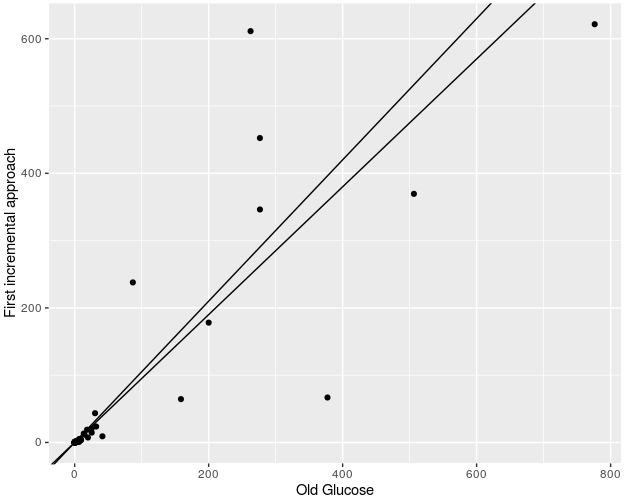
\includegraphics[scale=0.6]{img/glu_vs_incr1_dba.png}
 \caption{Graph comparing both minDBA time of minimization}
 \label{fig:glu_vs_incr1_dba}
\end{figure}

\begin{figure}[H]
 \centering
 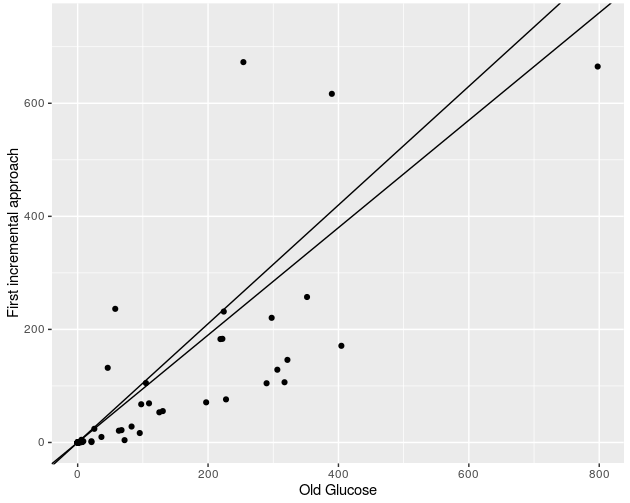
\includegraphics[scale=0.6]{img/glu_vs_incr1_dtgba.png}
 \caption{Graph comparing both minDTGBA time of minimization}
 \label{fig:glu_vs_incr1_dtgba}
\end{figure}

\noindent In light of the above, this incremental approach does not seem to be the most appropriate method.
This is really surprising. Why all that the SAT solver learned while solving the first traditional encoding
did not help him to solve quickly the next similar problems?\\

An hypothesis raised is that may be the fact that the size of the problem is never decreased affect it? By
restarting the encoding from scratch at each step, the Old SAT-based minimization also restarts with a
smaller automaton. The smaller the input automaton is, the smaller the SAT problem produced is (with a
decreasing number of litterals and clauses).